\section{Appendix: View Points}
\label{sec:appendix_view_points} 

This section defines how the view point files have to be structured and written by view point generators (applications which generate such files). \\

View point files are written in the JSON format, and includes a version number. The current version number is 0.2, the previous version 0.1 is \textbf{not} supported. \\

Please \textbf{note} that basic JSON format knowledge is required to understand the topics in this section. \\

Please \textbf{note} that the format definition has to be fulfilled rigorously, otherwise the application may not show the view point or (in rare cases) crash. \\

Please \textbf{note} that two different use cases were considered: a general one and one for tracker run comparison. The latter has additional parameters defined, to be used only in such circumstances.

\subsection{File Content}

The following content is commonly stored in a view point file:
 \begin{itemize}
 \item View points context information
 \begin{itemize}
 \item Information about all later view points
 \item Defines version
 \item Can be used for importing the relevant data files
 \item Also giving contextual information
 \end{itemize}
 \item View point collection, each consisting of information about
 \begin{itemize}
 \item Unique identifier
 \item View Point type
 \item Description text
 \item A point in time with a time window
 \item A position with a position window
 \item A list of DSTypes to be loaded
 \item A list of data sources to be loaded
 \item A list of filters
 \item A list of context variables
 \item A list of displayable annotations
  \end{itemize}
 \end{itemize}

\subsection{Custom Attributes}
\label{sec:view_points_custom_attributes} 

The view point context, as well as view points, can contain additional information. For the context, this additional information is shown in the 'Import View Points' task and not stored. \\

Additional data in each view point is read in as is, and persisted in the database. In the 'View Points' tab, all primitive variables (non-object, non-list) are shown as columns. \\

Therefore, when generating view points, it might be useful to add such variables (e.g. for ordering according to error magnitude, priority etc.). This is recommended and will be supported further.
 
\subsection{Version 0.2}

The most simple example of a view points file is as follows:

\lstset{
    string=[s]{"}{"},
    stringstyle=\color{blue},
    showstringspaces=false,
}
\begin{lstlisting}[basicstyle=\small\ttfamily]
{
    "content_type": "view_points",
    "content_version": "0.2",
    "view_points": [
        {
            "id": 1,
            "name": "All",
            "status": "open",
            "type": "Saved"
        }
    ]
}
\end{lstlisting}
%\ \\

There is an encompassing JSON object, which contains the view point context (object) and view points (list with one entry). \\

\subsubsection{View Point Context}

The 'version' attribute is mandatory, and only version 0.2 is currently supported. \\

In the context, optinally datasets can be added, which define related data to be imported.

\begin{lstlisting}[basicstyle=\small\ttfamily]
{
    "content_type": "view_points",
    "content_version": "0.2",
    "view_point_context": {
        "datasets": [
            {
                "filename": "/home/sk/data/test/asterix/test.ff"
            }
        ]
    },
    ...
}
\end{lstlisting}
%\ \\

Each dataset has to have a filename. \\

Several datasets are also possible:
\begin{lstlisting}[basicstyle=\small\ttfamily]
{
    "content_type": "view_points",
    "content_version": "0.2",
    "view_point_context": {
        "datasets": [
            {
                "filename": "/home/sk/data/test/asterix/test.ff"
            },
            {
                "filename": "/home/sk/data/test/asterix/test2.ff"
            },
            {
                "filename": "/home/sk/data/test/asterix/test3.ff"
            }
        ]
    },
    ...
}
\end{lstlisting}
%\ \\

Each of the defined ASTERIX datasets will be automatically imported when using the 'Import View Points' task. \\

Please note that the ASTERIX decoder settings have to be set correctly in the configuration and are the same for all files to be imported. \\

For the tracker run comparison case, additional attributes are used. The assumption is that there are two recordings, each containing a tracker run, each of which will be imported into a separate line. 
The tracker runs will possibly also have the same SAC/SIC and a time shift, which can be corrected during ASTERIX import using the features described in \nameref{sec:task_import_asterix_override}. \\

Such an import without overrides can look as follows:

\begin{lstlisting}[basicstyle=\small\ttfamily]
{
    "content_type": "view_points",
    "content_version": "0.2",
    "view_point_context": {
        "datasets": [
            {
                "filename": "/home/sk/data/test/asterix/test.ff",
                "line_id": 0,
                "date": "2021-01-02"
            },
            {
                "filename": "/home/sk/data/test/asterix/test2.ff",
                "line_id": 1,
                "time_offset": -60
            }
        ]
    },
    ...
}
\end{lstlisting}
%\ \\

In this case, the first dataset will be imported into line L1 (0 as L1, default line) with a date '2021-01-02', 
while the second dataset will be imported in to L2 and time shifted by the 'time\_offset' (as Time of Day in seconds). \\

Exact definition:

\begin{center}
 \begin{table}[H]
  \begin{tabularx}{\textwidth}{ | l | X | c | X | }
    \hline
    \textbf{Key} & \textbf{Value Description} & \textbf{Required} & \textbf{Comment} \\ \hline
    filename & File path and name (absolute) as string & Y & Needed for import \\ \hline
    line\_id & Line ID to be used during ASTERIX import & & \\ \hline
    time\_offset & ASTERIX tod offset as reference time minus dataset time, as number in seconds & & \\ \hline
\end{tabularx}
\end{table}
\end{center}
%\ \\

\subsubsection{View Point}

View points are stored in the 'view\_points' attribute, which is a simple list. \\

A view point only has to contain and 'id' and 'type' attribute, but additional attributes make it more meaninful.

\begin{lstlisting}[basicstyle=\small\ttfamily]
{
        ...
        {
            "id":0,
            "type":"any string",
            "text":"any string",
            "position_latitude":49.5,
            "position_longitude":12.2,
            "position_window_latitude":0.05,
            "position_window_longitude":0.02,
            "time":666.0,
            "time_window":4.0,
            "data_sources": [
                [
                    12750,
                    [
                        0,
                        1
                    ]
                ],
                [
                    12759,
                    [
                        2,
                        3
                    ]
                ]
            ],
            "data_source_types": [
                "Radar",
                "RefTraj"
            ],
            "filters": {
                "Time of Day": {
                    "Time of Day Maximum": "16:02:00.00",
                    "Time of Day Minimum": "16:00:00.00"
                },
                "UTNs": {
                    "utns": "4"
                }
            },
            "context_variables": {
                "Meta": [
                    "Ground Bit",
                    "Track Groundspeed"
                ]
            }
        },
        ...
}
\end{lstlisting}

In each View Point object, the following values can be defined:

\begin{center}
 \begin{table}[H]
  \begin{tabularx}{\textwidth}{ | l | X | c | }
    \hline
    \textbf{Key} & \textbf{Value Description} & \textbf{Required} \\ \hline
    id & Identifier, as number & Y \\ \hline
    type & Type, as string, e.g. 'Short track', 'Extra track', 'Content deviation X' & Y   \\ \hline
    text & Description text as string &    \\ \hline
    position\_latitude & Center position WGS-84 latitude, as number &    \\ \hline
    position\_longitude & Center position WGS-84 longitude, as number &    \\ \hline
    position\_window\_latitude & Geographic window size in WGS-84 latitude, as number &    \\ \hline
    position\_window\_longitude & Geographic window size in WGS-84 longitude, as number &    \\ \hline
    time & Center time, as number in seconds &    \\ \hline
    time\_window & Time window size, as number in seconds &    \\ \hline
    data\_sources & List of data sources to load, with lists which lines to load &    \\ \hline
    data\_source\_types & List of DSTypes to load, as strings &    \\ \hline
    filters & List of filters defining which data to load, as JSON objects &   \\ \hline
    context\_variables & List of extra content data variables to load and display &    \\ \hline
\end{tabularx}
\end{table}
\end{center}
%\ \\

If the 'data\_sources', 'data\_source\_types' or 'filters' attribute are not defined, all data will be loaded.

\subsubsection{View Point Filters}

The 'filters' attribute contains a JSON object, where each filter name is used as a key, and the value is again an JSON object encompassing the filter conditions. Each filter condition value is a string, the same as a user would enter in the GUI.

\begin{lstlisting}[basicstyle=\small\ttfamily]
{
        ...
        {
            ...
            "filters": {
                "Filter Name 1": {
                    "Filter Condition 1": "Value 1"
                },
                "Filter Name 2": {
                    "Filter Condition 1": "Value 1",
                    "Filter Condition 2": "Value 2"
                }
                ...
            }
            ...
        },
        ...
}
\end{lstlisting}      

When a view point is set, only the filters that are defined will be activated, all others will be disabled. If no 'filter' is defined, filtering will be disabled (load all data). \\

All possible filters existing in COMPASS can be set using view points, e.g.:

\begin{lstlisting}[basicstyle=\small\ttfamily]
{
        ...
        {
            "data_source_types": [
                "Other",
                "RefTraj",
                "Tracker"
            ],
            "filters": {
                "ADSBMOPS": {
                    "ADSBMOPSCondition0": "0"
                },
                "Aircraft Address": {
                    "Aircraft Address Values": "3cc0c4"
                },
                "Aircraft Identification": {
                    "Aircraft Identification Values": "teh01,teh08"
                },
                "Detection Type": {
                    "Radar Detection TypeCondition0": "1"
                },
                "Mode 3/A Codes": {
                    "Mode 3/A Codes Values": "4547"
                },
                "Mode C Codes": {
                    "Barometric Altitude Maximum": 24210.0,
                    "Barometric Altitude Minimum": 230.0,
                    "Barometric Altitude NULL": false
                },
                "Position": {
                    "Latitude Maximum": "49.215488",
                    "Latitude Minimum": "46.208428",
                    "Longitude Maximum": "17.335926",
                    "Longitude Minimum": "11.246144"
                },
                "Timestamp": {
                    "Timestamp Maximum": "2022-10-20 16:07:59.264",
                    "Timestamp Minimum": "2022-10-19 15:37:58.116"
                },
                "Track Number": {
                    "Track Number Values": "4547"
                },
                "Tracker Track Number": {
                    "Values": {
                        "12990": {
                            "0": "4171",
                            "1": "4281",
                            "2": "4197"
                        }
                    }
                }
            },
            "id": 3,
            "name": "sk",
            "position_latitude": 44.925597197536945,
            "position_longitude": 10.942831791785709,
            "position_window_latitude": 3.955006961478041,
            "position_window_longitude": 5.390988117653051,
            "status": "open",
            "type": "Saved"
        }
        ...
}
\end{lstlisting}

The filter values have to be defined exactly as a user would enter them in the DBFilter conditions in the GUI. \\

One exception are the data source filters, which need a 'active\_sources' condition list with integer values for all sources to be loaded, identified as number. Each source number is calculated by $SAC*255+SIC$. \\

For the 'Tracker Track Number' filter, the data source condition is identified by its data source name. Using the dataset in the context information, the view point file can ensure that the same name is used. \\

Please \textbf{note} that setting custom filters (created by the user) is also possible using view points. Please contact the author for further information.

\subsubsection{View Point Annotations}

The 'annotations' attribute stores custom geometry information, which can be displayed in an OSGView. \\

A simple example is shown below.

\begin{lstlisting}[basicstyle=\small\ttfamily]
{
        ...
        "annotations" :
        [
            {
                "name": "Point Annotation", 
                "symbol_color" : "#0000FF",
                "hidden": false,
                "features":
                [
                    // List of features contained in the annotation 
                    {
                        "type": "feature",
                        "geometry" :
                        {
                            "type": "points",
                            "coordinates": 
                            [
                                [45.0, 18.0], [46.0, 19.0], [45.0, 20.0], [48.0, 20.0]
                            ]
                        },
                        "properties":
                        {
                            "color": "#FF0000",
                            "symbol": "square",
                            "symbol_size": 24
                        }
                    }    
                ]
            }
        ]
        ...
}
\end{lstlisting}

An annotation obtains: \\

\begin{itemize}
    \item 'name': Display name of the information.
    \item 'symbol\textunderscore color': Color of the displayed annotation symbol in hex code.
    \item 'hidden': The annotation should be displayed in OSGView's layer tree.
    \item 'features': A list of features, describing displayable information. \\
\end{itemize}

Loading a viewpoint containing the example above will result in OSGView displaying the contained visual information,
a set of point coordinates in this case. In addition, the created annotation is shown in OSGView's layer tab under the node \textit{Annotations}.
A listed annotation can be shown or hidden by using the checkbox next to it. \\

\textbf{Note} how the chosen 'name' and 'symbol\textunderscore color' reflect in the displayed annotation node.

\begin{figure}[H]
    \center
      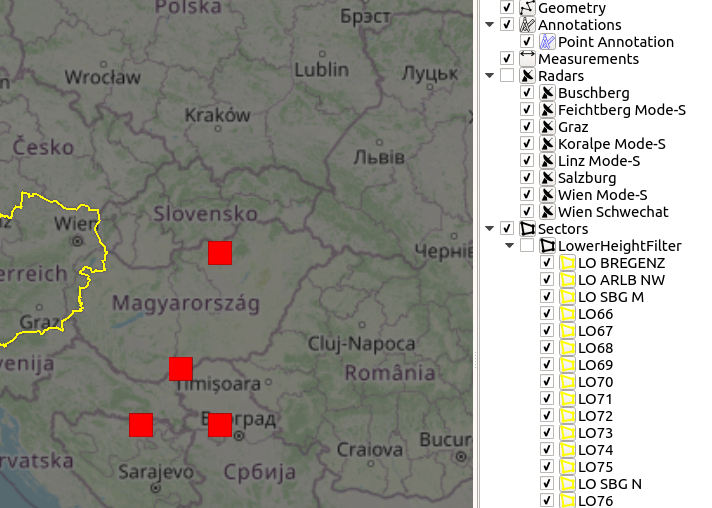
\includegraphics[width=12cm]{figures/viewpoints_anno_example.png}
    \caption{View Point Annotations - Example} 
\end{figure}

Examples for the existing 'features' will be given below.

\paragraph{Points} The 'points' feature displays a set of coordinates using a specified symbol.

\begin{lstlisting}[basicstyle=\small\ttfamily]
{
        ...
        {
            "type": "feature",
            "geometry" :
            {
                "type": "points",
                "coordinates": 
                [
                    [45.0, 18.0], [46.0, 19.0], [45.0, 20.0], [48.0, 20.0]
                ]
            },
            "properties":
            {
                "color": "#FF0000",    // Color of the symbols in hex code
                "symbol": "square",    // Symbol to be displayed, possible values 'square', 'cross', 'triangle' or 'circle'   
                "symbol_size": 24      // Display size of the symbol
            }
        }
        ...
}
\end{lstlisting}

\begin{figure}[H]
    \center
      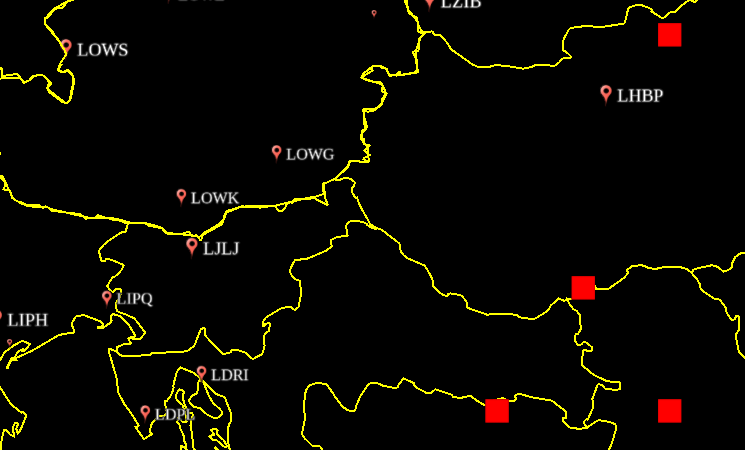
\includegraphics[width=8cm]{figures/viewpoints_anno_example_points.png}
    \caption{View Point Annotations - Points} 
\end{figure}

\paragraph{Lines} The 'lines' feature displays an array of lines. 
Two consecutive coordinates hereby form an individual line, which means that the size of the coordinate array needs to be even.

\begin{lstlisting}[basicstyle=\small\ttfamily]
{
        ...
        {
            "type": "feature",
            "geometry":
            {
                "type": "lines",
                "coordinates": 
                [
                    [45.0, 18.0], [45.0, 20.0], [48.0, 20.0], [46.0, 19.0]
                ]
            },
            "properties" :
            {
                "color": "#FFFFFF",  // Color of the displayed lines in hex code
                "line_width": 3.5    // Width of the displayed lines
            }
        }
        ...
}
\end{lstlisting}

Here $[45.0, 18.0]$ and $[45.0, 20.0]$ form one line, and $[48.0, 20.0]$ and $[46.0, 19.0]$ another one.

\begin{figure}[H]
    \center
        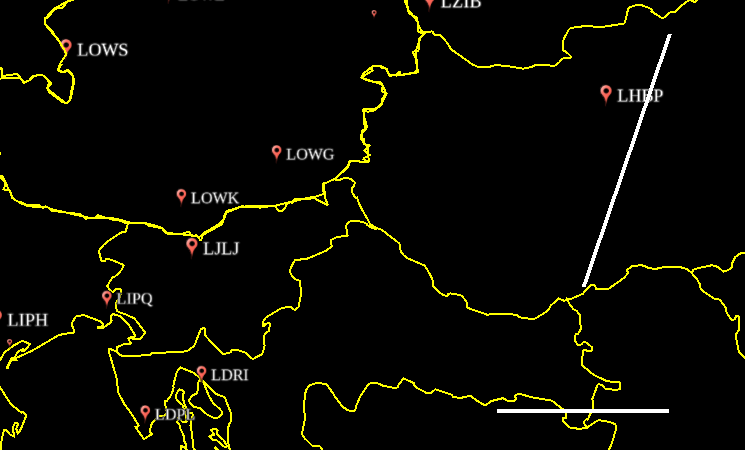
\includegraphics[width=8cm]{figures/viewpoints_anno_example_lines.png}
    \caption{View Point Annotations - Lines} 
\end{figure}

\paragraph{Line Strings} The 'line\textunderscore string' feature displays a polygonal line connecting the provided coordinates.

\begin{lstlisting}[basicstyle=\small\ttfamily]
{
        ...
        {
            "type": "feature",
            "geometry" :
            {
                "type": "line_string",
                "coordinates": 
                [
                    [45.0, 18.0], [46.0, 19.0], [45.0, 20.0], [48.0, 20.0]
                ]
            },
            "properties":
            {
                "color": "#0000FF", // Color of the displayed lines in hex code
                "line_width": 1.5   // Width of the displayed lines
            }
        }
        ...
}
\end{lstlisting}

The displayed line connects the given coordinates, one after another.

\begin{figure}[H]
    \center
        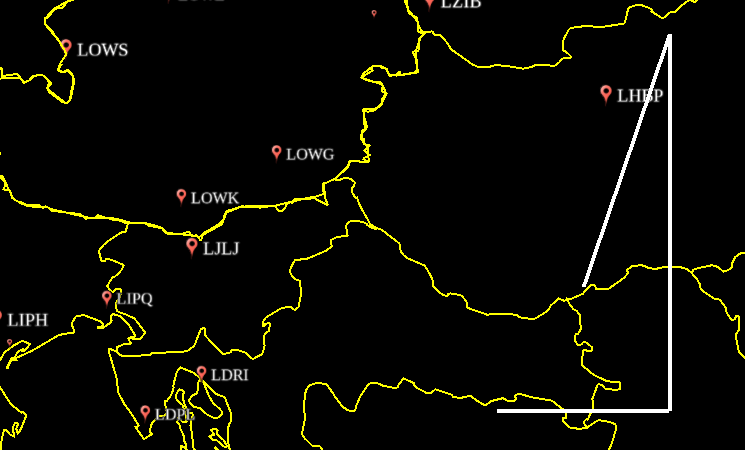
\includegraphics[width=8cm]{figures/viewpoints_anno_example_linestring.png}
    \caption{View Point Annotations - Line Strings} 
\end{figure}

\paragraph{Ellipses} The 'ellipses' feature displays accuracy information as ellipses at the provided locations.

\begin{lstlisting}[basicstyle=\small\ttfamily]
{
        ...
        {
            "type": "feature",
            "geometry":
            {
                "type": "ellipses",
                "coordinates": 
                [
                    [44.0, 14.0], [44.0, 16.0], [47.0, 16.0], [45.0, 15.0]
                ],
                "sizes": 
                [
                    [10000.0, 20000.0, 1500000], [20000.0, 30000.0, 300000000], [50000.0, 60000.0, 50000433], [80000.0, 90000.0, 2]
                ]
            },
            "properties" :
            {
                "color": "#0000FF",
                "line_width": 2.7,
                "num_points": 32     // Number of points used to approximate an ellipsis
            }
        }
        ...
}
\end{lstlisting}

The 'sizes' of the ellipses are provided as value triples (Standard deviation X, Standard deviation Y, Covariance XY).

\begin{figure}[H]
    \center
        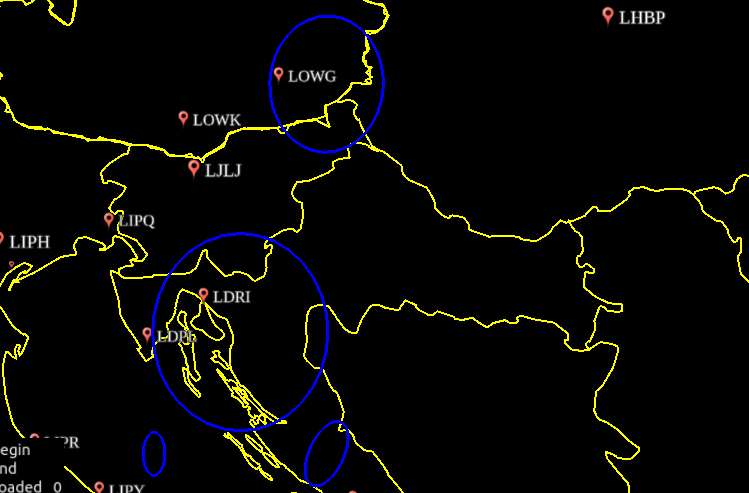
\includegraphics[width=8cm]{figures/viewpoints_anno_example_ellipses.png}
    \caption{View Point Annotations - Ellipses} 
\end{figure}

\paragraph{Text} The 'text' feature displays a text box at a provided coordinate.

\begin{lstlisting}[basicstyle=\small\ttfamily]
{
        ...
        {
            "type": "text",
            "text": "My Text",
            "position": [12.0, 22.0],     // A single coordinate
            "properties":
            {
                "color": "#AA00FF",       // Text color in hex code
                "direction": "left-up",   // Alignment of the text relative to the provided coordinate, possible values 'right-up', 'right-down', 'left-up' or 'left-down'
                "font_size": 10           // Displayed font size
            }    
        }
        ...
}
\end{lstlisting}

\begin{figure}[H]
    \center
        
\includegraphics[width=10cm]{figures/viewpoints_anno_example_text.png}
    \caption{View Point Annotations - Text} 
\end{figure}

\textbf{Note} that coordinates always need to be provided as WGS84 latitude and longitude. \\

\paragraph{Showing Color Arrays} In all examples provided above, a single color has been used for the geometry stored in a feature.
In order to show each geometrical primitive in a separate color, the 'color' tag can be removed, and a 'colors' array provided instead.

\begin{lstlisting}[basicstyle=\small\ttfamily]
{
        ...
        {
            "type": "feature",
            "geometry" :
            {
                "type": "points",
                "coordinates": 
                [
                    [45.0, 18.0], [46.0, 19.0], [45.0, 20.0], [48.0, 20.0]
                ],
                "colors": [ "#AA00FF", "#AA66FF", "#AAAAFF", "#AAEEFF"]
            },
            "properties":
            {
                "symbol": "square",
                "symbol_size": 24
            }
        }
        ...
}
\end{lstlisting}

This example will result in each point to be displayed in a separate color.

\begin{figure}[H]
    \center
        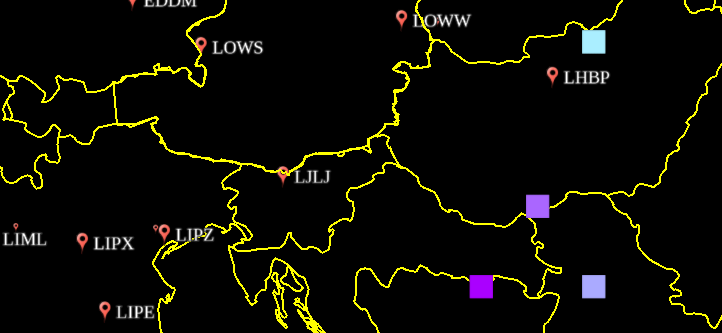
\includegraphics[width=8cm]{figures/viewpoints_anno_example_colorvec.png}
    \caption{View Point Annotations - Color vectors} 
\end{figure}

\textbf{Note}: A 'color' tag and a 'colors' array may not exist in a feature at the same time.

\paragraph{Nesting Annotations} Annotations can be nested by providing them with their own 'annotations' array containing nested 
annotations, as shown in the example below. This mechanism can be used to form more complex annotations, which can be switched on and off 
individually.

\begin{lstlisting}[basicstyle=\small\ttfamily]
{
        ...
        "annotations" :
        [
            {
                "name": "Group1",
                "symbol_color" : "#0000FF",
                "annotations" :                  // Annotations inside an annotation
                [
                    {
                        "name": "Nested annotation 1",
                        "symbol_color" : "#0000FF",
                        "features":
                        [
                            {
                                "type": "text",
                                "text": "Nested annotations are nice",
                                "position": [12.0, 22.0],
                                "properties":
                                {
                                    "color": "#0000FF",
                                    "direction": "left-up",
                                    "font_size": 10
                                }
                            }
                        ]
                    }
                ]
            },
            {
                "name": "Group2",
                "symbol_color" : "#FF00FF",
                "annotations" :                // More Annotations inside an annotation
                [
                    {
                        "name": "Nested annotation 2",
                        "symbol_color" : "#FF00FF",
                        "features":
                        [
                            {
                                "type": "text",
                                "text": "Nested annotations are nice",
                                "position": [14.0, 24.0],
                                "properties":
                                {
                                    "color": "#FF00FF",
                                    "direction": "left-up",
                                    "font_size": 10
                                }
                            }
                        ]
                    }
                ]
            }                
        ]
        ... 
}
\end{lstlisting}

\begin{figure}[H]
    \center
        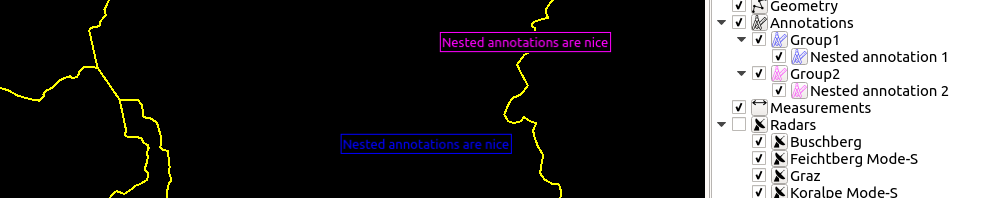
\includegraphics[width=14cm]{figures/viewpoints_anno_example_nested.png}
    \caption{View Point Annotations - Nested Annotations} 
\end{figure}
